\begin{frame}
	\frametitle{Nomes não descritivos}

	\begin{figure}[h]
		\centering
			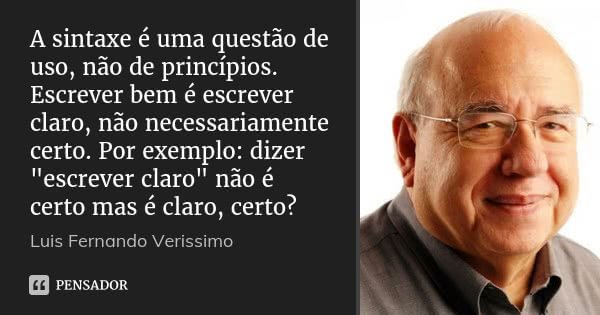
\includegraphics[height=0.6\paperheight]{figuras/luis}
		\caption{Retirada do site \href{https://www.pensador.com/frase/MTU0NjQ/}{Pensador}}\label{figure:luis}
	\end{figure}

\end{frame}

\begin{frame}
	\frametitle{Problemas}
	\begin{itemize}
		\item Não saber o que a função faz de fato
		\item Dificuldade em encontrar erros
		\item Necessidade de olhar a implementação
	\end{itemize}
\end{frame}

\begin{frame}
	\Huge Caso real
\end{frame}

\begin{frame}[fragile]

	\begin{listing}[H]
		\caption{Código em C $\sharp$}
		\begin{minted}[baselinestretch=1.2,fontsize=\scriptsize,linenos]{csharp}
private void tabPage1_Click(object sender, EventArgs e);

private void dateTimePicker2_ValueChanged(object sender, EventArgs e);
	\end{minted}
	\end{listing}

\end{frame}

\begin{frame}
	\Huge Caso real
\end{frame}

\begin{frame}[fragile]
	\frametitle{Função \textit{resolve}}

	\begin{listing}[H]
		\begin{minted}[baselinestretch=1.2,fontsize=\scriptsize,linenos]{c}
double resolve(char *n){
	char op='\0',a[100]={'\0'},b[100]={'\0'},op2='\0',xc[100]={'\0'},dpa[100]={'\0'};
	int j,po=0,tam,l,v=0,po2=0,v2=0,co=0,k,cof=0,coa=0,poa=0,pof=0,dp=0,t=0;
	double ai=0,bi=0,ri=0;
	tam=strlen(n);
	//...
}
		\end{minted}
	\end{listing}
\end{frame}

\begin{frame}[fragile]

	{\Huge Sabe o significado da variável \textit{po}?}

\end{frame}

\begin{frame}[fragile]

	{\Huge Sabe o significado da variável \textit{po}?}\\
	Posição do primeiro operador

\end{frame}

\begin{frame}
	\Huge Exemplo
\end{frame}

\begin{frame}[fragile]
	\frametitle{O que essa função faz?}

	\begin{listing}[H]
		\caption{Declaração da função}
		\begin{minted}[baselinestretch=1.2,fontsize=\scriptsize,linenos]{c}
		float calc (float b, float c);
	\end{minted}
	\end{listing}

\end{frame}

\begin{frame}

	\Huge Que significado a função \textit{calc} tem?

\end{frame}

\begin{frame}[fragile]
	\frametitle{Agora você sabe? Mas o que o nome dela te diz?}

	\begin{listing}[H]
		\caption{Implementação da função}
		\begin{minted}[baselinestretch=1.2,fontsize=\scriptsize,linenos]{c}
float calc (float b, float c){
	float a = b * c;
	return a;
}
		\end{minted}
	\end{listing}

\end{frame}

\begin{frame}

	{\Huge Que significado a função \textit{calc} tem?}
	\begin{itemize}
		\item É uma função para multiplicar dois valores?
		\item É uma função para calcular a área de um retângulo?
	\end{itemize}
\end{frame}

\begin{frame}[fragile]
	\frametitle{O que essa função faz?}

	\begin{listing}[H]
		\caption{Declaração da função de multiplicar}
		\begin{minted}[baselinestretch=1.2,fontsize=\scriptsize,linenos]{c}
float multiplicar (float primeiroValor, float segundoValor);
		\end{minted}
	\end{listing}

\end{frame}

\begin{frame}[fragile]
	\frametitle{Versão melhorada da função \textit{calc}}

	\begin{listing}[H]
		\caption{Código em C}
		\begin{minted}[baselinestretch=1.2,fontsize=\scriptsize,linenos]{c}
float multiplicar (float primeiroValor, float segundoValor){
	float resultado = primeiroValor * segundoValor;
	return resultado;
}
		\end{minted}
	\end{listing}

\end{frame}

\begin{frame}
	\Huge Exemplo
\end{frame}

\begin{frame}[fragile]
	\frametitle{O que essa função faz? O que t representa?}

	\begin{listing}[H]
		\begin{minted}[baselinestretch=1.2,fontsize=\scriptsize,linenos]{python}
def getT():
	return t / 60;
		\end{minted}
	\end{listing}

\end{frame}

\begin{frame}[fragile]
	\frametitle{O que essa função faz? O que tempo representa?}

	\begin{listing}[H]
		\begin{minted}[baselinestretch=1.2,fontsize=\scriptsize,linenos]{python}
def getTempo():
	return tempo / 60;
		\end{minted}
	\end{listing}

\end{frame}

\begin{frame}[fragile]
	\frametitle{Ainda tem dúvida sobre o que a função faz?}

	\begin{listing}[H]
		\begin{minted}[baselinestretch=1.2,fontsize=\scriptsize,linenos]{python}
def getTempoEmMinutos():
	return tempoEmSegundos / 60;
		\end{minted}
	\end{listing}

\end{frame}

\begin{frame}
	\Huge Exemplo
\end{frame}

\begin{frame}[fragile]
	\frametitle{O que essa função faz?}

	\begin{listing}[H]
		\caption{Código para logar no sistema SIGA}
		\begin{minted}[baselinestretch=1.2,fontsize=\scriptsize,linenos]{python}
def loginSiga(username, password):
		#...
		\end{minted}
	\end{listing}

\end{frame}

\begin{frame}[fragile]

	\begin{listing}[H]
		\caption{Código para logar no sistema SIGA}
		\begin{minted}[baselinestretch=1.2,fontsize=\scriptsize,linenos]{python}
def loginSiga(username, password):
	driver = webdriver.PhantomJS()
	driver.set_window_size(1024, 768) # optional
	driver.get('https://sistemas.ufscar.br/siga/')

	formularioLogin = driver.find_element_by_id("login")
	campoUsuario = driver.find_element_by_name("login:usuario")
	campoSenha = driver.find_element_by_name("login:password")
	botaoLogin = driver.find_element_by_name("login:j_idt39")

	#...

	return toJSON(driver.page_source.encode('ascii', 'ignore'))
		\end{minted}
	\end{listing}

\end{frame}


\begin{frame}
	\frametitle{Solução}
	\begin{itemize}
		\item Escolha um nome que descreva o que a função faz
		\item Os nomes das variáveis devem expressar significado
		\item Evite usar siglas
	\end{itemize}
\end{frame}
